
\subsection{Global camera calibration}
\label{sec:global-calib}


To calibrate the multi-camera system, we follow the common framework that consists of searching for feature point correspondences and minimizing re-projection errors.
%
Because of the lack of the features in indoor scenes and the high requirement of the quality of the calibration, we use a $6\times7$ checkerboard with squares of 117 mm which can be made easily for the accuracy and robustness.

%
An user holding the checkerboard could move in front of the cameras freely in the working space.
At each moment, the 8 cameras capture images simultaneously.
%
The checkerboard is simultaneously seen in three or four views usually.
%
Our system is flexible enough while it does not require that the checkerboard must be visible under all points of view.
%
We also use the images with checkerboard on the ground which allows the checkerboard corners can be seen in all the 8 cameras, as shown in Figure~\ref{fig:checkerboard}.
This will help to reduce the accumulative error and inconsistence caused by the pairwise calibration.
\begin{figure}[ht]
%
\begin{minipage}[b]{.48\linewidth}
  \centering
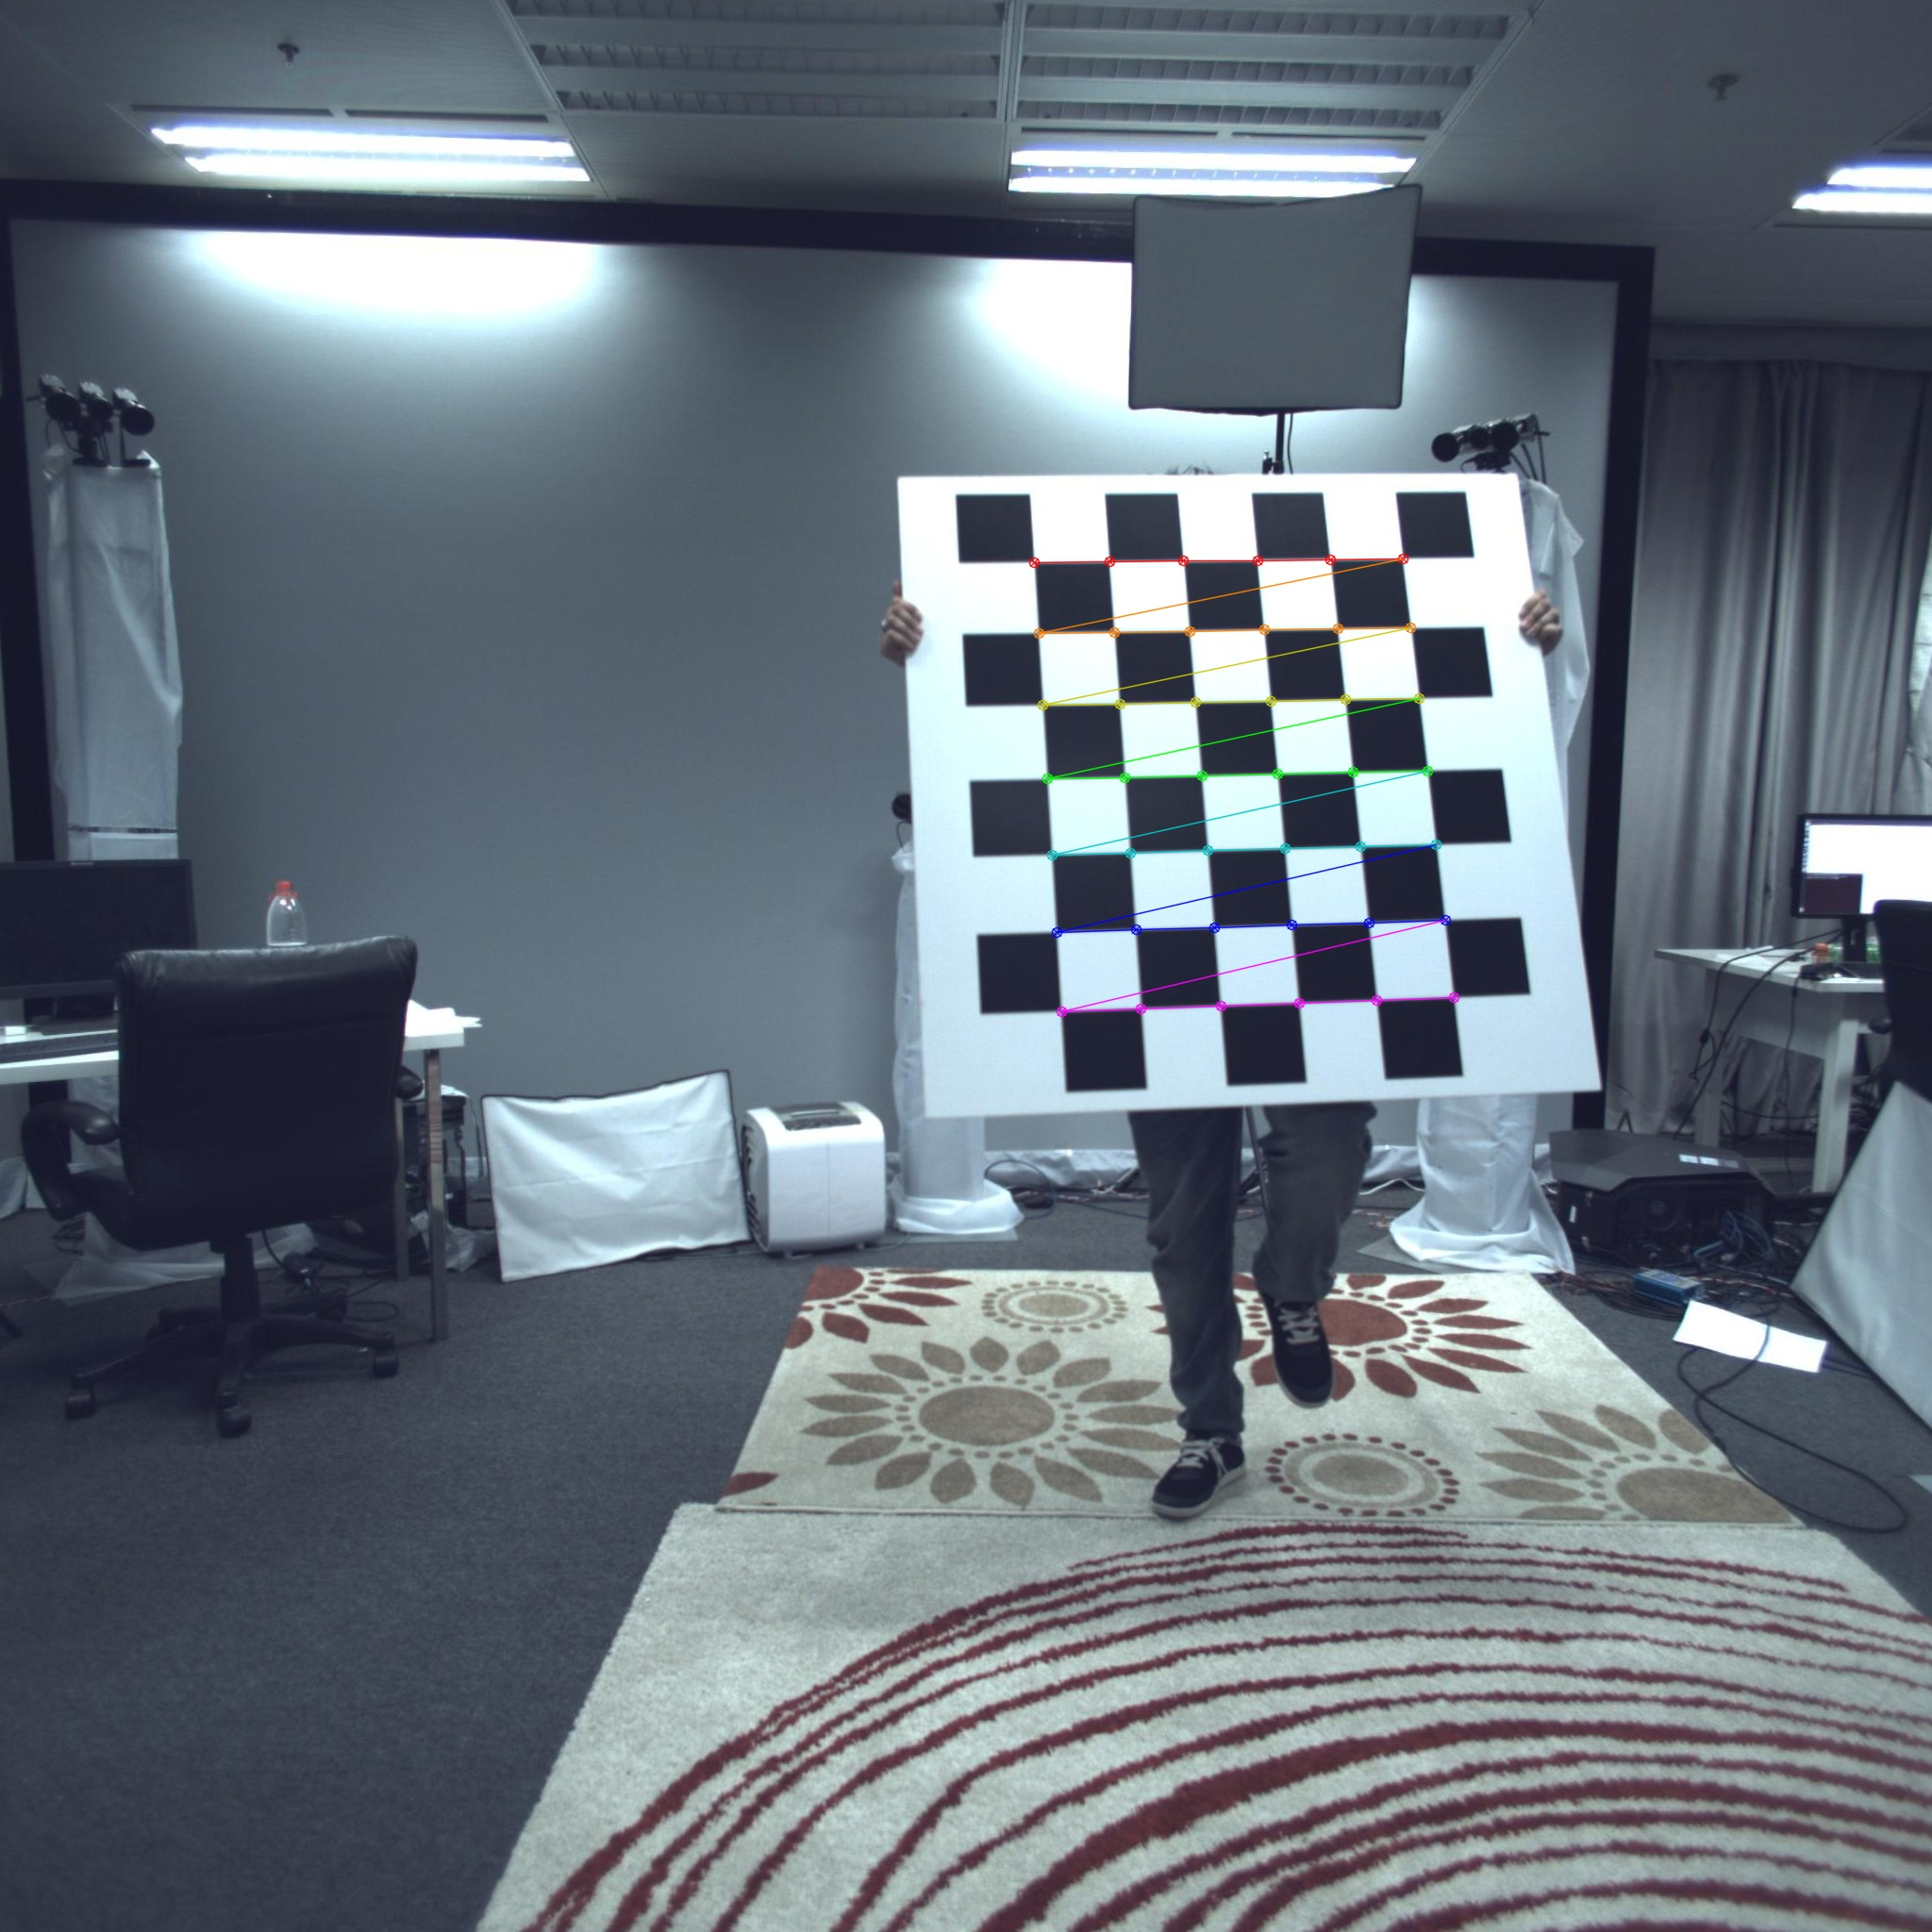
\includegraphics[scale=0.058]{image/free.jpg}
  \vspace{0cm}
  \centerline{(a)}\medskip
\end{minipage}
\hfill
\begin{minipage}[b]{0.48\linewidth}
  \centering
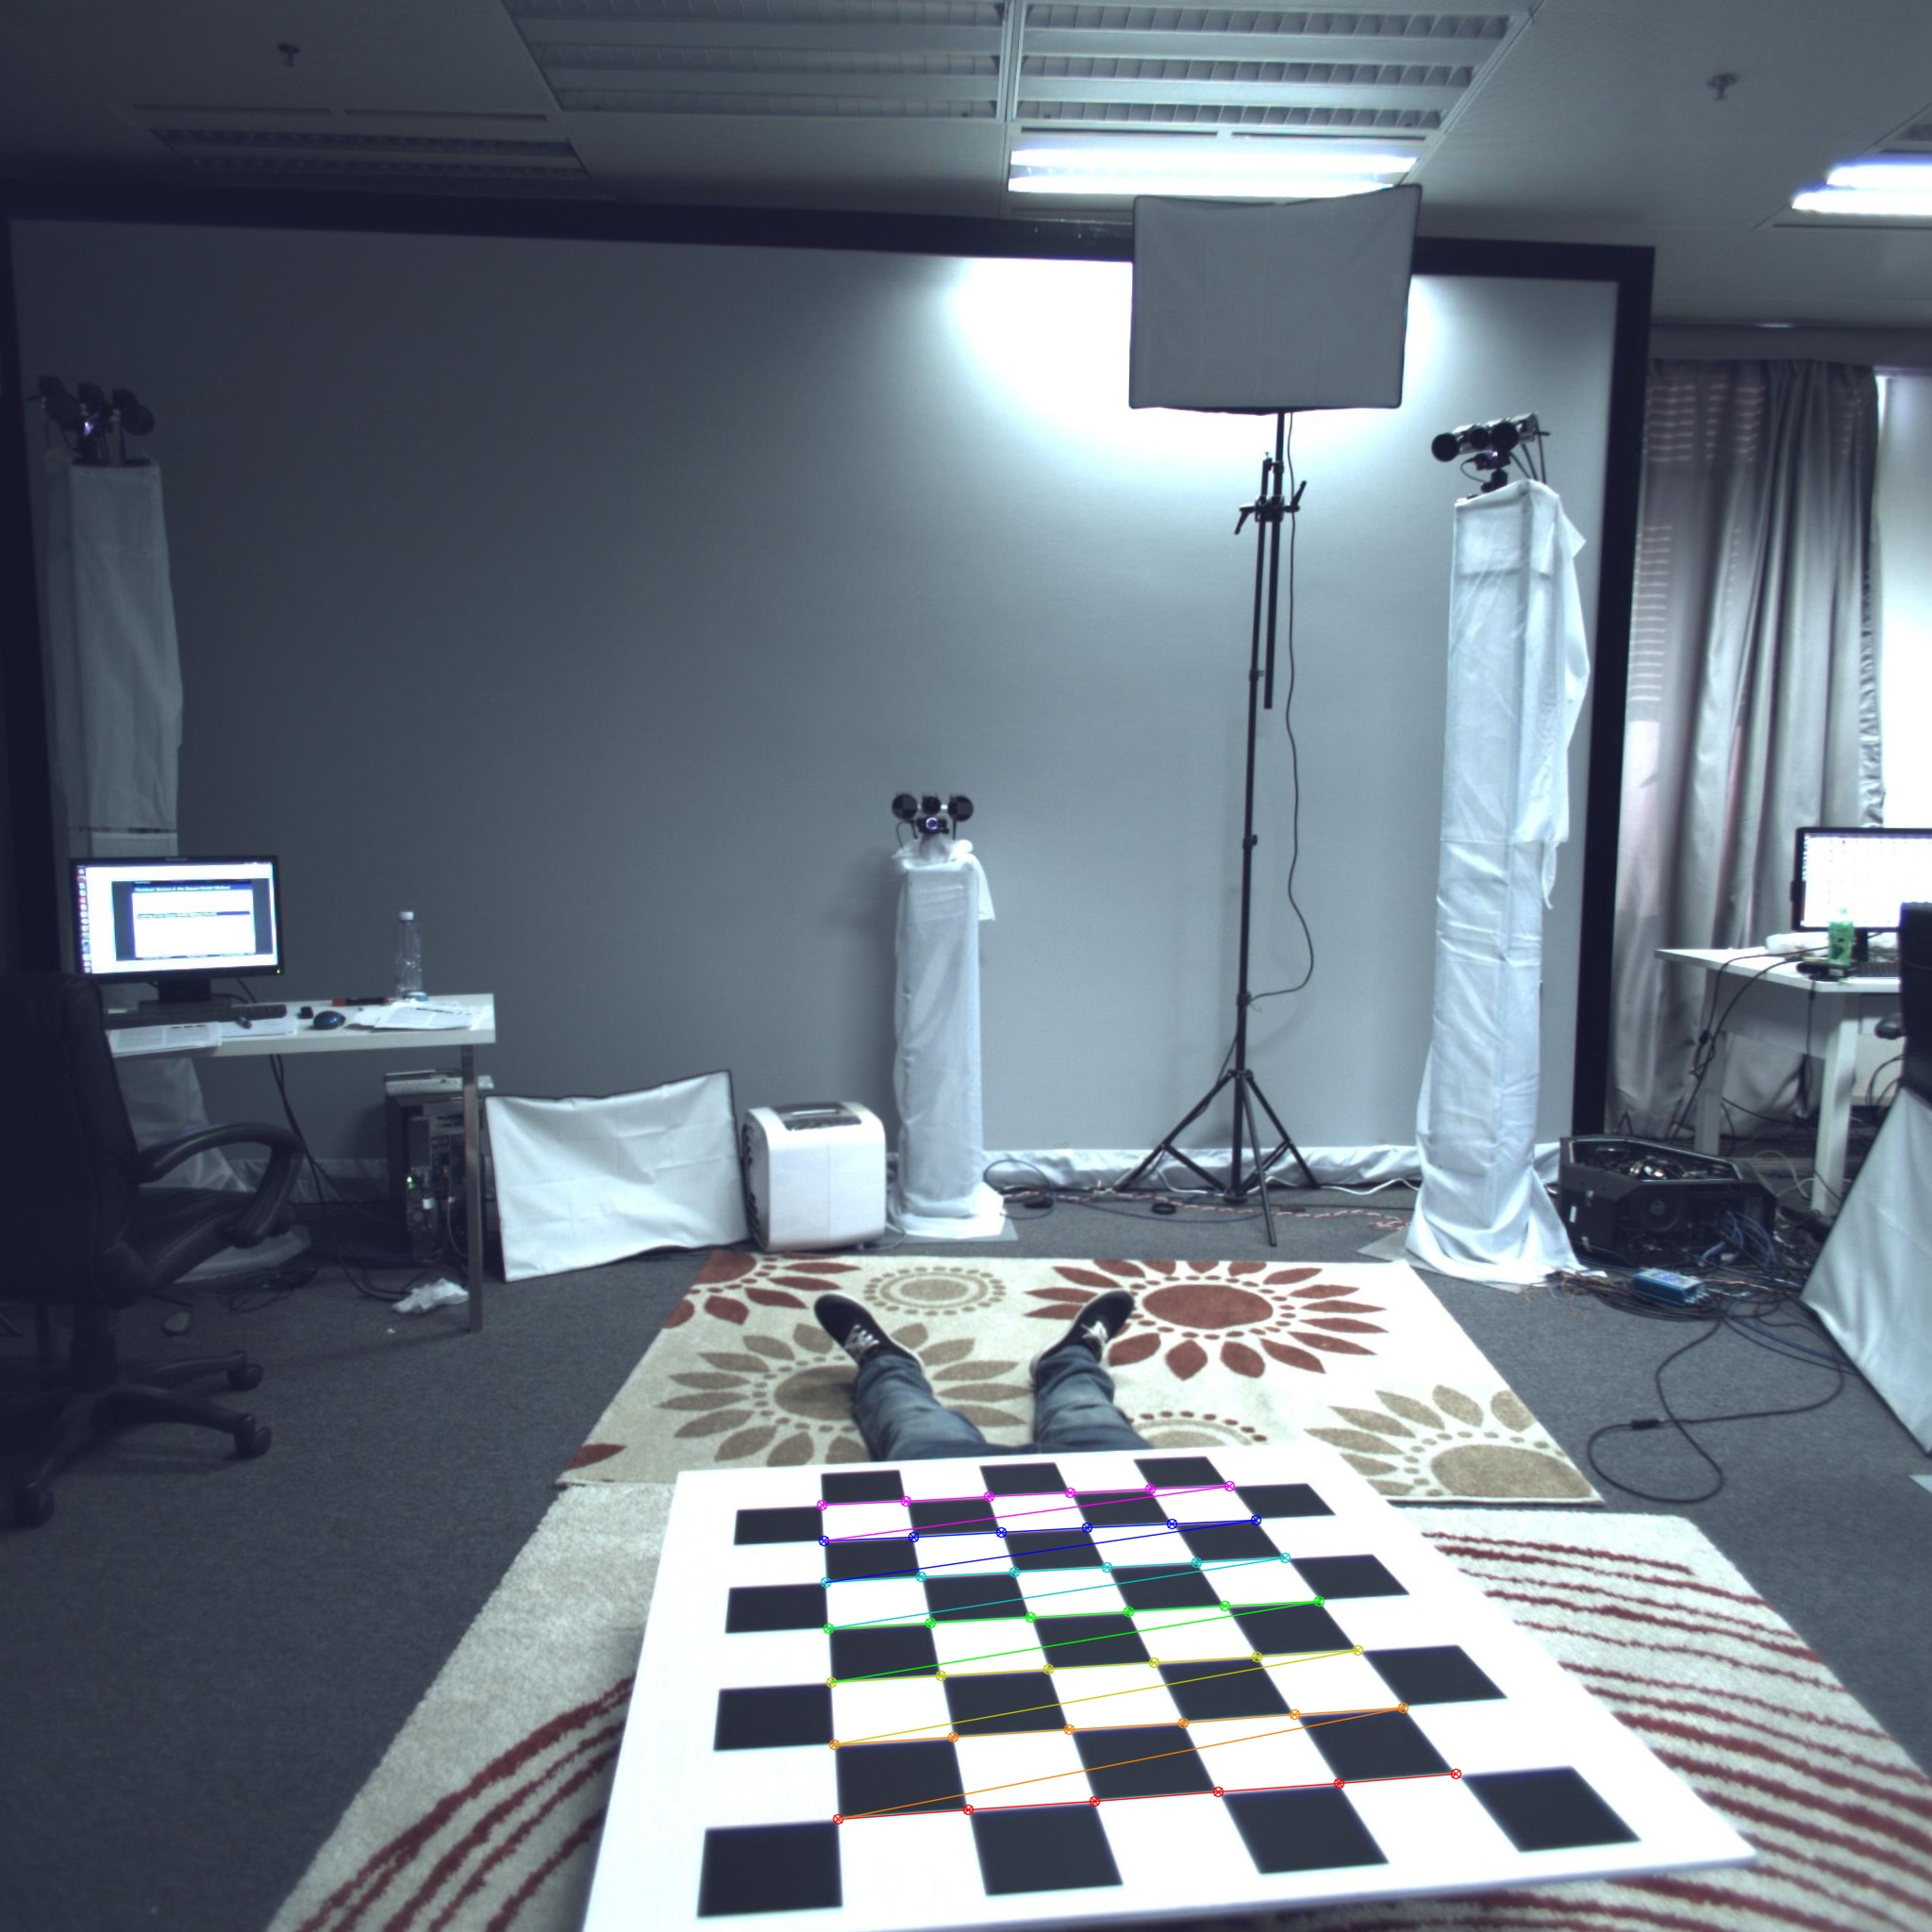
\includegraphics[scale=0.058]{image/ground.jpg}
  \vspace{0cm}
  \centerline{(b)}\medskip
\end{minipage}
%
\caption{Results of the checkerboard corners detection. (a): Results when the user moves freely. (b): Results when the checkerboard is on the ground. }
\label{fig:checkerboard}
\end{figure}
%
Then the 42 corners on the checkerboard can be detected in each local group.
%
For each time $t$, denote the group of cameras that can see the checkerboard corners as $\mathcal{C}^t$. The 3D coordinates of the 42 corner points are denoted as $\{\vb{p}^{t}_{i}\}_{i=1,\ldots, 42}$, while their corresponding 2D coordinates detected in each image captured by the camera $c_j \in \mathcal{C}^{t}$ are $\{\vb{x}^{t}_{ji}\}$.
%
While the user holding the checkerboard moves around, we can capture $T$ groups of checkerboard images and combine them together to globally estimate the camera parameters.
%


According to the re-projection equation defined in Eq.~\ref{eq:cam-proj}, our calibration method optimizes the camera parameters to minimize the re-projection errors. Considering the $T$ groups of images together, the re-projection error is defined as:
%
\begin{equation} \label{eq:global-proj-error}
E(\mathbf{M}_{j},\mathbf{p}^{t}_{i})=\sum_{t}\sum_{j\in \mathcal{C}^{t}}\sum_{i} \big( \hat{\vb{x}}(\vb{K}_{j},\mathbf{M}_{j}, \vb{p}^{t}_{i})-\mathbf{x}^{t}_{ji} \big)^{2},
\end{equation}
%
where $\hat{\vb{x}}(\vb{K}_{j},\mathbf{M}_{j}, \mathbf{p}_{i})$ is the estimated 2D positions of a 3D point $\vb{p}^{t}_{i}$ in the image plane of the camera $c_j$ with its parameters $\camin_j$ and $\camex_j$.


The above optimization could be solved by the Sparse Bundle Adjustment package~\cite{lour09}, which uses a Levenberg-Marquardt technique to optimize the parameters iteratively.
Inevitably, this algorithm only finds a local optimal.
A good initialization is required to get a good results.


Though sequentially calibrating the neighboring cameras leads to accumulated errors, it could provide an initialization for the global optimization.
%
We use the toolbox Kalibr~\cite{Maye2013Self} to obtain the intrinsic parameters and the initial extrinsic parameters of neighboring cameras sequentially.
%
Then we estimate the 3D coordinates $\mathbf{p}^{t}_{ji}$ of each corner from the corresponding 2D coordinates by triangulation.
%where $n$ is the number of the views that the checkerboard can be seen in at the same time.
%
After the initial calibration, we globally optimize the extrinsic parameters and the 3D coordinates of each corner.
Typically, $T=30$ groups produce good enough results.

The re-projection error describes the accuracy of the calibration system.
We compute the average re-projection error and compare it to evaluate the effectiveness of our global calibration step.
%
Using the 2D coordinates of the corners detected in the checkerboard images, we can achieve the 3D space coordinates of $\mathbf{p}^{t}_{i}$ by triangulation respectively using the camera parameters obtained by Kalibr and our global calibration method.
Then we re-project $\mathbf{p}^{t}_{i}$ to each view which the checkerboard can be seen and compute the average re-projection error, as shown in Table~\ref{tab:reprojection}.


\begin{table*}
	\centering
	\caption{Average re-projection error (pixels) of each camera using different methods. (a) results by Kalibr~\cite{Maye2013Self}, (b) results by our global calibration method. The re-projection error of (b) is smaller and uniform in each view, while the results of (a) contain the accumulative error and the inconsistence. }
	\label{tab:reprojection}
	\begin{tabular}{lcccccccc}
		\hline
		Methods & Cam 1 & Cam 2 & Cam 3 & Cam 4 & Cam 5 & Cam 6 & Cam 7 & Cam 8\\
		\hline
		(a) Kalibr &4.54 &3.20 &11.16 &10.74 &4.87 &6.75 &3.64 &5.11\\
		
		(b) SBA   &\textbf{0.32} &\textbf{0.32} &\textbf{0.38}  &\textbf{0.35} &\textbf{0.37} &\textbf{0.40} &\textbf{0.33} &\textbf{0.34} \\
		
		\hline
		
	\end{tabular}


\end{table*}
%As shown in Fig.~\ref{fig:}, the projected error ...
%\xj{Show a figure to compare the reprojected points before/after SBA.}\md{To Do}

%\subsection{Multi-camera system}

\comments{
We employ 8 camera pods around the working space looking inwards for a full capture as shown in Figure~\ref{fig:rig}. Each camera pod consists of one color camera and two Near Infra-Red cameras. A laser pointer is used to produce special patterns.
From the two images of the projected patterns captured by the two NIR cameras, a depth map can be estimated using PatchMatch stereo algorithm~\cite{Bleyer2011PatchMatch}.
% it depth images can be achieved by the 2  using depth estimation methods.


%\subsection{Camera model}
Let $\mathbf{p}=(x,y,z,1)^{T}$ be the homogeneous coordinate of a point $P$ in the 3D space, and $\mathbf{x}=(u,v,1)^{T}$ the homogeneous coordinates of its projected point on an image plane, the perspective re-projection of a pin-hole camera is usually described as
\begin{equation}
z_{p}\mathbf{x}=\mathbf{K}\mathbf{M}\mathbf{p},
\end{equation}
where $z_{p}$ is the projective depth of point $P$, $\mathbf{K}$ and $\mathbf{M}$ are the intrinsic and extrinsic parameters of the camera.



%\subsection{Initial calibration}
The $\mathbf{K}$ and initial $\mathbf{M}$ of each camera are calibrated by Kalibr~\cite{Maye2013Self} pairwisely because of the lack of the common overlapping fields of view, including the 8 color cameras' extrinsic parameters $\{\mathbf{M}_{i}\}_{i=1,\ldots,8}$. The extrinsic parameters from the 2 NIR cameras to the color camera in the same camera pod are also achieved, but these extrinsic parameters are fixed and used to estimate the depth in each view.
}

%\subsection{Global optimization}








